\chapter{Felhasznált technológiák}

A fejezet célja, hogy bemutassa a videó streaming szolgáltatások implementációjához felhasznált konkrét szoftvereket, webes és felhőszolgáltatásokat, és az azok közötti kapcsolatokat.

\section{FFMpeg szoftvercsomag}

Az FFMpeg\footnote{\url{https://www.ffmpeg.org/}} egy nyílt forráskódú és GPL-licenszelésű szoftvercsomag, amely képes videók és hangok kódolására, dekódolására, átalakítására (konvertálás), valamint streamelésre. \cite{ffmpeg} Az FFMpeg a legtöbb operációs rendszeren elérhető, és számos különböző formátumot, modern kodekeket támogat. Az FFMpeg a videók és hangok kódolására és dekódolására szolgáló kodekeket tartalmazza, valamint számos különböző formátumot támogat, beleértve az MPEG-4, H.264, H.265, VP8, VP9, AV1, AAC, AC-3, Opus, és sok más formátumot. Folyamatosan frissen tartják a kodekeket, aktív fejlesztőbázissal rendelkezik.

A lokális videókonvertálásra és streamelésre az FFMpeg-csomagból az azonos nevű ffmpeg parancssori interfészt használtam. Beépítettem a webszerver alkalmazásba egy külön szolgáltatásrészt, amely kihív a webszerver folyamatából és egy megfelelően felparaméterezett ffmpeg parancsot futtat a videókonvertálásra és streamelés megkezdésére aszinkron módon, a kimeneti fájlokat a megfelelő helyre menti.

A felhőalapú megoldásban már nem került felhasználásra az FFMpeg, mivel az AWS Elemental szolgáltatásokat használtam a videókódolásra és streamelésre, viszont a szoftvercsomag közvetlen megismerése a videókonvertálás folyamatának megértését és a konvertálási folyamatok felparaméterezési lehetőségeinek mélyebb átlátását segítette.

\section{Open Broadcaster Software}

Az Open Broadcaster Software Studio (OBS Studio\footnote{\url{https://obsproject.com/}}) egy nyílt forráskódú, szabad szoftver, amelyet elsősorban élő közvetítésekhez és képernyőrögzítéshez használnak. Elterjedt Twitch-felhasználók körében. A program támogatja a Windows, macOS és Linux operációs rendszereket, és számos beállítási lehetőséget biztosít a felhasználók számára. Az OBS lehetővé teszi több videó- és hangforrás kombinálását, ennek köszönhetően webkamera felvétele, mikrofon inputja, az éppen használt képernyő képe vagy előre rögzített videók is kombinálhatóak a stúdió műszerfalán.

A szoftver kompatibilis a legnépszerűbb streamingplatformokkal, így például a YouTube-ra és a Twitchre is lehet feltölteni vele, és lehetőséget biztosít saját egyedi RTMP-szerverekhez való csatlakozásra is annak felkonfigurálásával. Az OBS Studio megbízható eszköz azok számára is, akik professzionális szintű élő közvetítést szeretnének megvalósítani.

\section{Amazon Web Services}

Az Amazon Web Services (AWS) a világ egyik legjobban elterjedt, legnagyobb szerverfarmjait fenntartó, nagy hírű vállalatok által is megbízható felhőszolgáltatója. Felhasználói számára számítási, hálózati, adattárolási célokat megvalósító szolgáltatások széles palettáját kínálja. Felhasználják az AWS-t a mesterséges intelligencia területén; valamint kiterjedt adatbázisok, adatfeldolgozó rendszerek építésére; megbízható és könnyen skálázható webes szoftverrendszerek kialakítására.

A felhasználók a szolgáltatásokhoz az AWS Management Console webes felületen keresztül, vagy az AWS Command Line Interface (AWS CLI) parancssori interfészén keresztül férhetnek hozzá. Az egyes felhasználók fel tudnak állítani maguknak egy vagy több AWS-fiókot, amelyek a számlázás és a jogosultságkezelés szempontjából elkülönülhetnek egymástól.

A fiókon belül lehetőséget kapunk granuláris jogosultságkezelésre, azaz az egyes felhasználók, szolgáltatások, vagy szolgáltatásrészek számára különböző alacsony szintű jogosultságokat adhatunk meg.

Az AWS regionális adatközpontokat üzemeltet a világ számos pontján, amelyek közül a felhasználók választhatnak, hogy melyik adatközpontban szeretnének szolgáltatásokat futtatni.

A költségeket ``pay-as-you-go'' alapelv alapján számolják fel, azaz a felhasználók csak az általuk használt szolgáltatások számítási kapacitásáért, a tárhelyért, az adatközpontból kifelé történő hálózati forgalomért fizetnek.

\subsection{AWS Elemental}

Az Elemental Technologies 2006-ban indította vállalkozását streamingmegoldások eladására, egy fő mérföldkövük volt, amikor a szolgáltatásaikkal került közvetítésre a 2012-es nyári olimpiai játékok Londonban. Az Elemental Technologies 2015-ben került az Amazon Web Services tulajdonába, azóta az AWS Elemental néven futó szolgáltatásokat kínálja az AWS-felhőben. A fő célja a szolgáltatáscsomagnak, hogy óriási célközönségek számára is megbízható streamközvetítési megoldásokat kínáljon, amelyeket könnyen lehet skálázni, és amelyek a legújabb videókódolásokat és -technológiákat alkalmazzák. \cite{Elemental}

Szoftveres megoldásaik közé tartoznak a következők: 

\begin{itemize}
  \item \textbf{Elemental MediaConvert}: A MediaConvert egy felhőalapú videókódoló szolgáltatás, Software-as-a-Serviceként viselkedik, egy API-t ad, amelyen keresztül kódolási munkafolyamatokat (``jobokat'') indíthatunk. A MediaConvert támogatja a legnépszerűbb videóformátumokat, mint például a H.264, H.265, és a VP9, valamint a legújabb HDR (High Dynamic Range) és Dolby Vision technológiákat is. HLS streamre is képes felkészíteni a videókat. Csupán fel kell tölteni a forrásvideót egy S3-vödörbe, majd a konvertálás után a kimeneti videók számára is egy S3-vödröt tudunk megadni.
  \item \textbf{Elemental MediaLive}: Az Elemental MediaLive egy élő videókódoló szolgáltatás, amely lehetővé teszi a felhasználók számára, hogy élő videóadásokat fogadjanak és kódoljanak át a felhőben. A MediaLive támogatja a legnépszerűbb élővideó feltöltési protokollokat, így az RTMP-t is. Ennek a használata már bonyolultabb, mint a MediaConverté, nem szimplán csak egy API meghívásaként kell elképzelni. Külön csatornákat lehet benne definiálni, azokhoz inputot/inputokat rendelni, ezután pedig a kódolási munkafolyamatokat felkonfigurálni. Az AWS sokféle nyelvben garantál SDK-kat, amelyek segítségével könnyen lehet automatizáltan MediaLive-csatornákat indítani külön-külön adásokhoz.
  \item \textbf{Elemental MediaPackage}: Az Elemental MediaPackage készíti elő, csomagolja a videófolyamot hálózati protokollokon szállítmányozásra, garantálja a biztonságos és folyamatos tartalomtovábbítást. Biztosíthatja VOD-ok S3-ból való továbbosztását, vagy élők továbbosztását a MediaLive-ból. A MediaPackage támogatja a legnépszerűbb kliensfelőli protokollokat, mint például az HLS, DASH és a Microsoft Smooth Streaming. Könnyedén integrálható CloudFront-disztribúciókba.
\end{itemize}

Érdemes még a szoftveres megoldások közt megemlíteni az Elemental MediaConnectet, amely egy Quality of Service (QoS) réteget biztosít a streamet fogadók és az AWS-felhő között, megbízható és biztonságos hálózati kapcsolatot biztosít. Ismert lehet még az Elemental MediaTailor, amely lehetővé teszi a reklámok beillesztését a videófolyamainkba. Korábban még a felhozatalba tartozott, azonban kivezetésre kerül már az Elemental MediaStore 2025. november 13-áig, amely egy objektumtároló szolgáltatás volt, viszont már az Amazon S3 kiváltotta, mivel az már erős read-after-write konzisztenciát tud biztosítani 2020 óta. \cite{Mediastore}

Ezeken kívül az AWS szolgáltat még fizikai hardvereket is a streaming könnyítésére és a nagy számításigények kiszolgálására, ezek közé tartozik például a AWS Elemental Link, amely egy HDMI- és SDI-portokkal rendelkező eszköz, lehetővé teszi a helyszíni videóforrások közvetlenül a felhőbe való továbbítását. A szoftveres és hardveres megoldások összekötésére egy példát szolgáltat mind VOD-ok és élő adások kiszolgálására a \refstruc{fig:vodlive}.

\begin{figure}
	\centering
	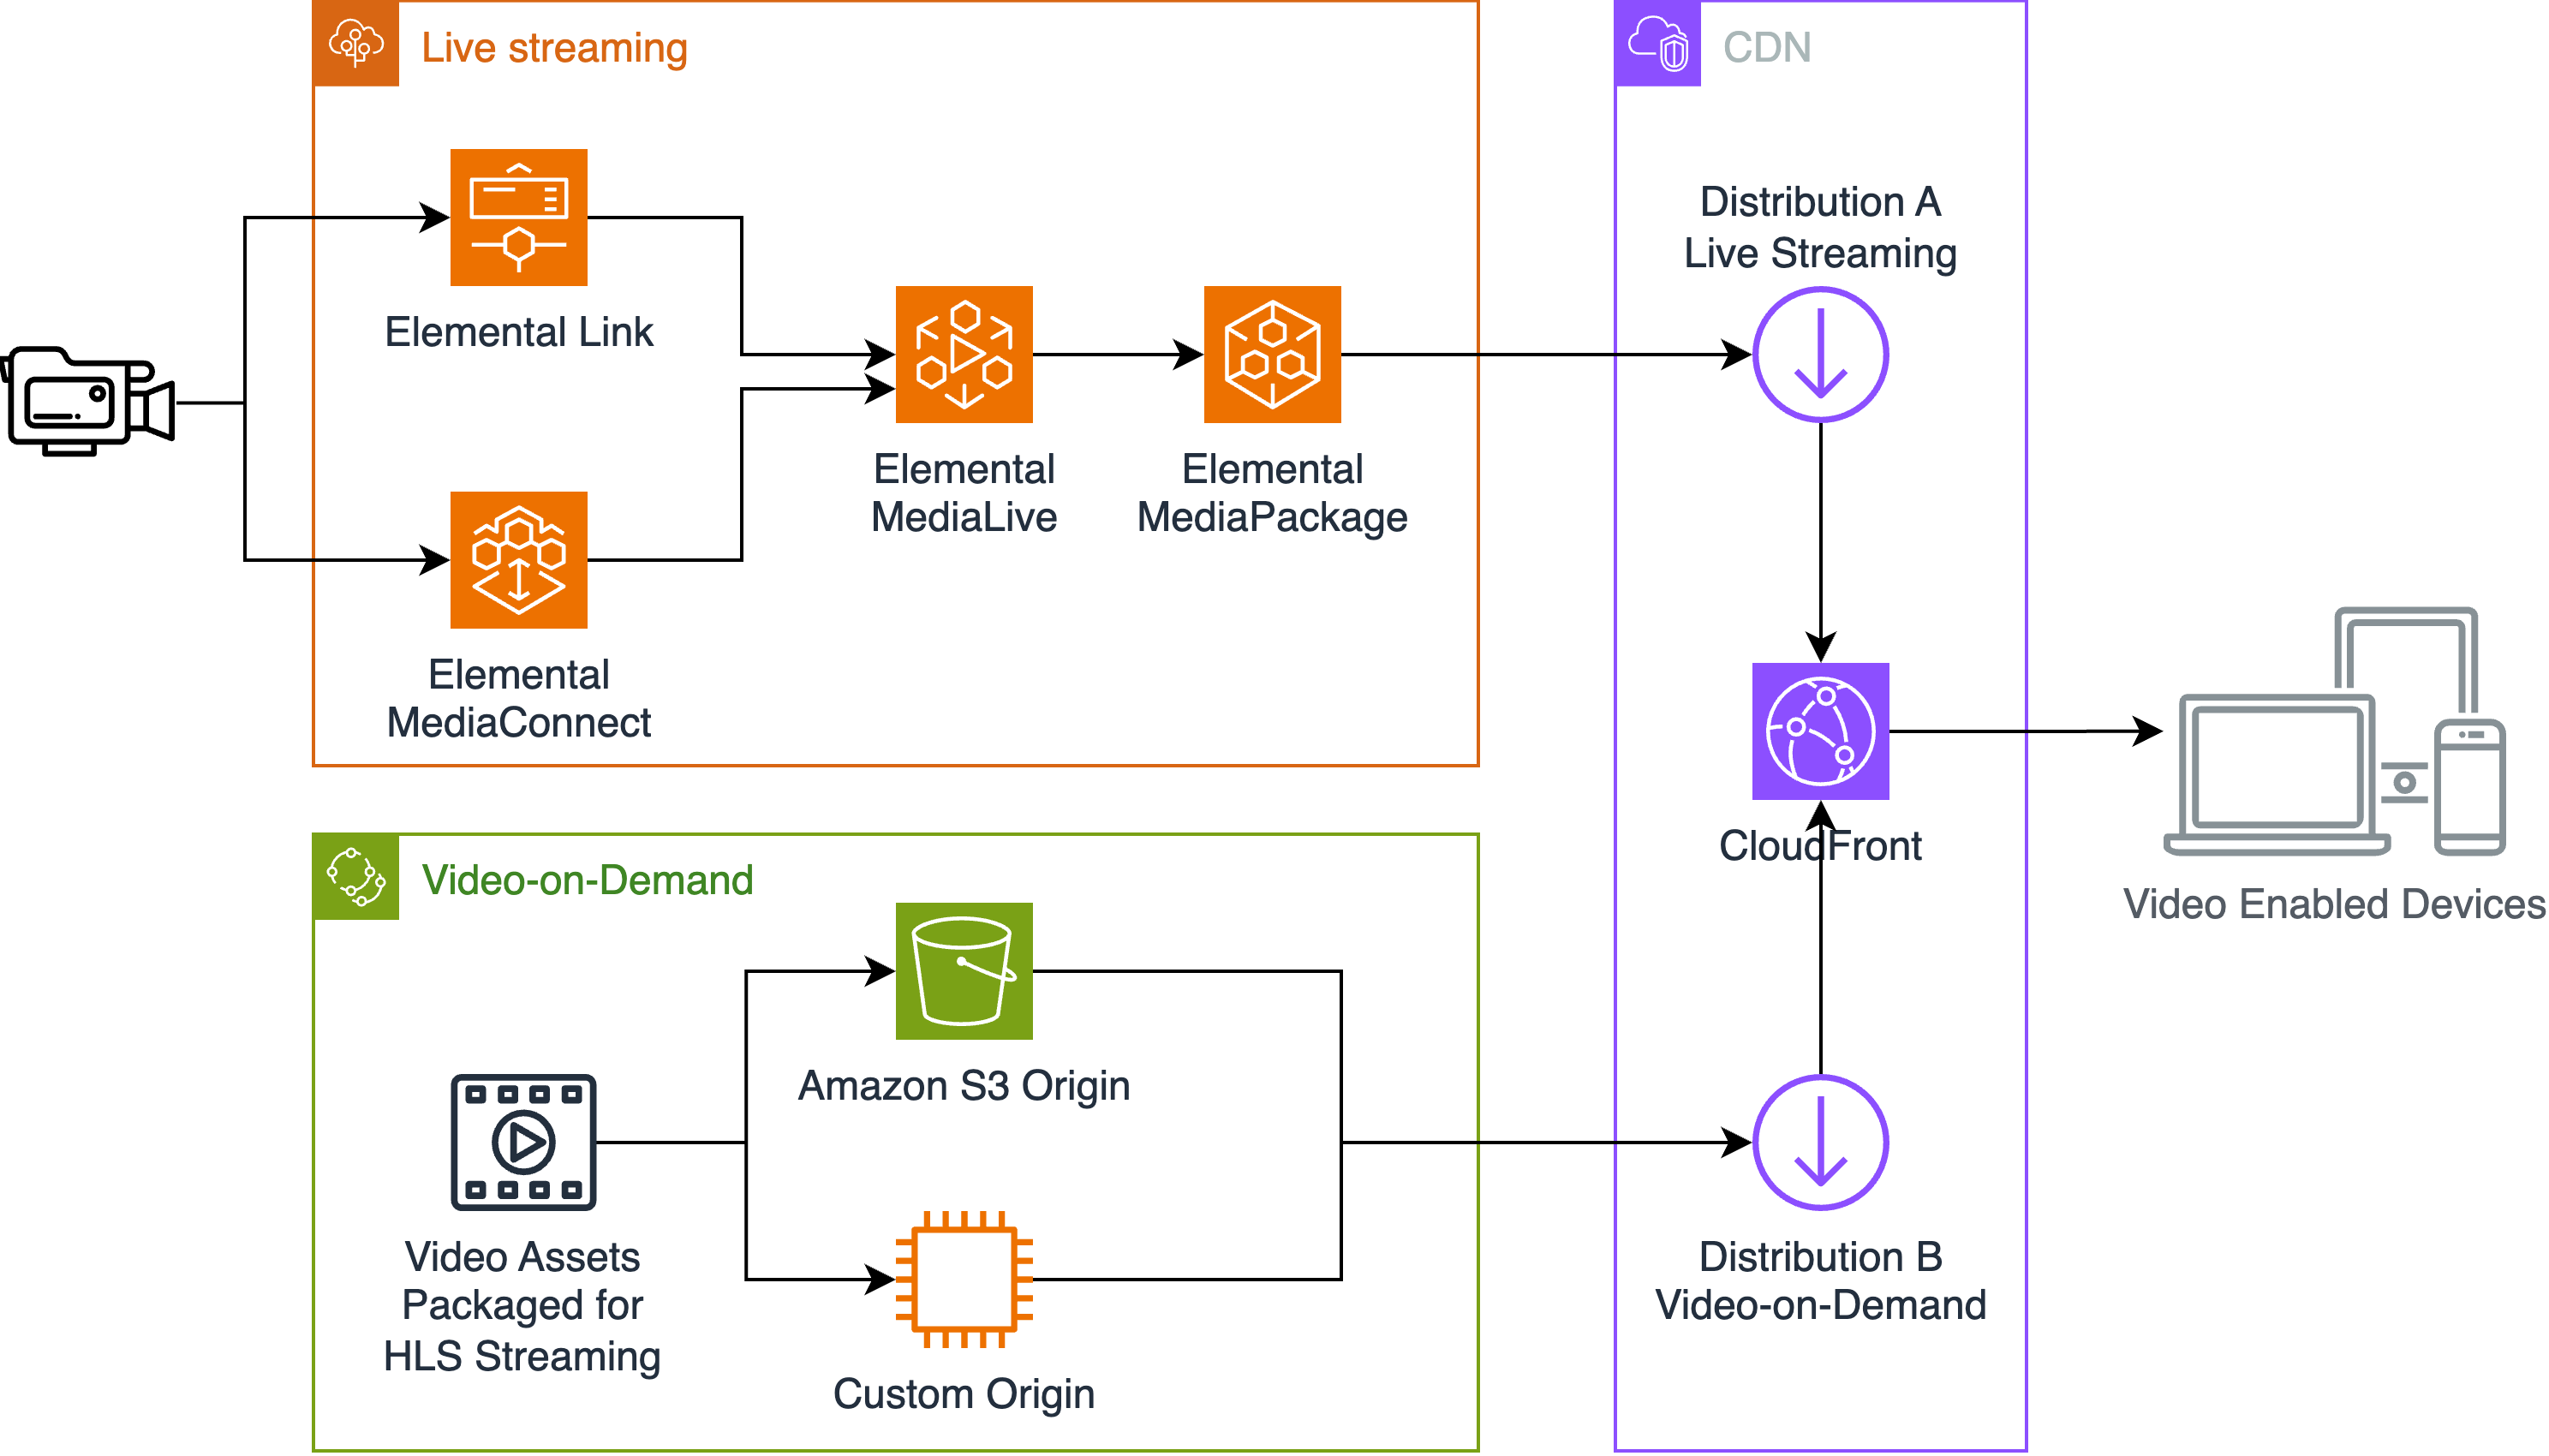
\includegraphics[width=120mm, keepaspectratio]{figures/dipterv_vodlive.png}
	\caption{Példa AWS Elemental szolgáltatások architektúrába kötésére.}
	\label{fig:vodlive}
\end{figure}

\subsection{Amazon IVS}

Az Amazon Interactive Video Service (IVS) egy teljesen AWS-kezelt, skálázható, és megbízható élő videó streaming Software-as-a-Service (SaaS), amely lehetővé teszi a fejlesztők számára, hogy gond nélkül integrálják az élő streaming funkcionalitását a saját alkalmazásaikba. Az IVS az Elemental szolgáltatásokhoz képest end-to-end megoldást kínál kis késleltetésű többnézős alkalmazásra: HLS-alapú kiszolgálás, körülbelül 5 másodperces késleltetést szokott biztosítani; valamint valós idejű alkalmazásra is: WebRTC-alapú kiszolgálás. \cite{Ivs} A forrásvideó-kódolástól a tartalomkiszolgálásig minden szükséges funkciót biztosít (\refstruc{fig:ivselemental}\footnote{A kép forrása: \url{https://aws.amazon.com/blogs/media/awse-choosing-aws-live-streaming-solution-for-use-case/}}), nekünk csupán a Software Development Kitjét (SDK) kell használni a saját alkalmazásunkban, és a többit az AWS-re bízhatjuk. Ezenkívül biztosít olyan funkcionalitásokat, mint chatszobák és szavazások szolgáltatása, amelyeket könnyen integrálhatunk ezekbe az adásokba.

\begin{figure}
	\centering
	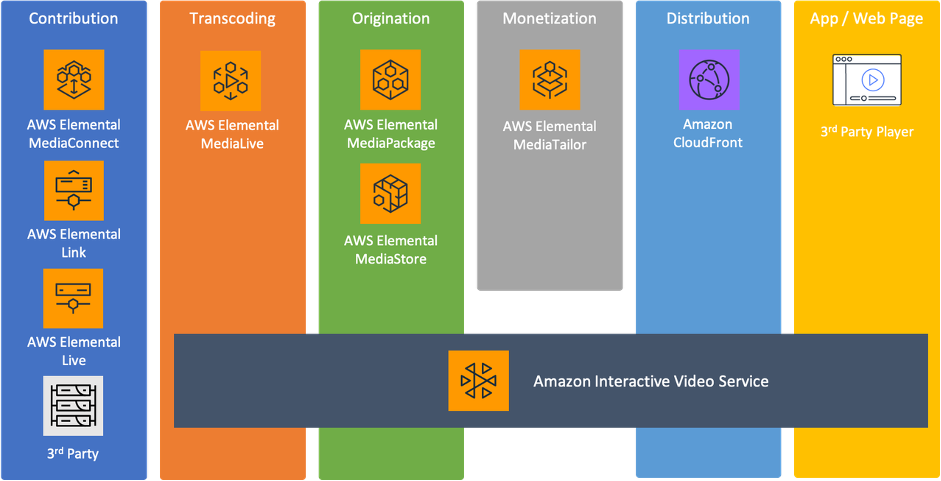
\includegraphics[width=120mm, keepaspectratio]{figures/aws_media.png}
	\caption{Amazon IVS és az AWS Elemental szolgáltatások összehasonlítása.}
	\label{fig:ivselemental}
\end{figure}

Ezen szolgáltatás ismertetése a megértést és a választás indoklását szolgálja későbbi fejezetekben, az Amazon IVS nem került felhasználásra a konkrét lefejlesztett rendszerben.

\subsection{Amazon VPC}

Az Amazon Virtual Private Cloud (Amazon VPC) egy virtuális hálózati környezet. Benne megvalósítható, hogy az AWS publikus felhőjén belül is privát és publikus saját hálózatokat hozzunk létre. Az Amazon VPC segítségével a felhasználók teljes kontrollt gyakorolhatnak a virtuális hálózati környezetük felett, beleértve a VPC-k alatti alhálózatok IP-tartományainak konfigurálását, útvonaltáblák kitöltését, a hálózati interfészek/portok korlátozásait, egyéb hálózati eszközök beillesztését (NAT Gateway-ek, Internet Gateway-ek, valamint Transit Gateway-ek), felülvizsgálható benne a hálózati teljesítmény.

Különféle eszközöket kínál a felhasználók számára, hogy biztonságossá tegyék az AWS-felhőn belüli hálózati környezetüket. Priváttá tehetik alhálózataik, bevezethetnek állapotmentes korlátozást ki- és bemenő forgalomra (engedélyezett IP-tartományok és portok megadásával), erre jók alhálózatokra alkalmazható Network Access Control Listek (NACL), vagy a konkrét erőforrásokra alkalmazható Security Groupok. Állapottartó megoldás az AWS Network Firewall. VPC Flow Logok bekötésével monitorozható válik a hálózati forgalom is.

\subsection{Amazon ALB}

Az Application Load Balancer (ALB) az Amazon Elastic Load Balancer (ELB) egy fajtája, ISO--OSI Layer 7 szinten, azaz alkalmazásrétegek szintjén működő terheléselosztó hálózati eszköz. Automatikusan skálázódik, lehetővé teszi a felhasználók számára, hogy egy vagy több szerver példány között egyenletesen eloszthassák a beérkező HTTP- és HTTPS-kéréseket. Az ALB képes a kéréseket a kérések fejlécei alapján vagy a kérések útvonala alapján elkülöníteni a forgalmat.

\subsection{Amazon S3}

Az Amazon Simple Storage Service (Amazon S3) egy objektumtároló szolgáltatás, amely lehetővé teszi a felhasználók számára, hogy nagy mennyiségű adatot tároljanak az AWS-felhőben ``vödrökben'' (bucketokban). Az objektum egy fájl és a fájlt leíró metaadatok közösen. A vödör az objektumok tárolója.

\subsection{Amazon CloudFront}

Az előző fejezet egy szekciójában már említetésre kerültek a CDN mint a Video-on-Demand alapú streaming szolgáltatások egyik kulcsfontosságú eleme. Az Amazon CloudFront egy globális CDN, amely lehetővé teszi a felhasználók számára, hogy a tartalmat hozzájuk közelebbi szervereken tárolt cache-ből töltsék le, ezáltal csökkentve a késleltetést, csökkentve a központi szerverek terhelését, és növelve a letöltési sebességet. Tartalmaink csoportosítására CloudFront-``disztribúciókat'' használunk.

A disztribúciók különböző URI-útvonalaikon akár különböző CDN-forrásokból -- úgynevezett ``originekből'' -- tudnak tartalmat kiszolgálni: ilyen origin lehet egy S3-vödör, AWS Elemental MediaPackage-alapú élő adást sugárzó csatorna, Amazon Application Load Balancer (ALB) példány, vagy akár egy egyéni HTTP-szerver is saját doménnévvel.

\subsection{Amazon ECS}

Az Amazon Elastic Container Service (ECS) arra szolgál, hogy konténeralapú alkalmazásokat, szoftvercsomagokat futtathassunk a felhőszolgáltatónál. Az ECS segítségével a felhasználók könnyen futtathatnak és skálázhatnak konténereket anélkül, hogy a konténerek futtatásához szükséges infrastruktúra mélyén futó szervergépeket, valamint azok életciklusát, operációs rendszerének patch-elését kellene kezelniük -- ezek menedzselését az AWS Fargate motor veszi át, mi csupán a környezeti paramétereket kell felkonfiguráljuk az igényeinknek megfelelően.

Ilyen paraméterek a konténerek képei, a konténerek alapvető számítási erőforrásai (CPU-magok száma, memória mérete), a konténerek hálózati beállításai (porttovábbítások, alkalmazott Security Group), a konténerek naplózása (hova továbbítódjanak a futtatás során a naplók), és a konténerek hozzáférési jogosultságai az AWS-felhőn belüli más szolgáltatásokhoz. Könnyedén kapcsolható össze Amazon ALB-példánnyal.

Tipikusan alkalmazott az ECS párban az Amazon Elastic Container Registry (ECR) szolgáltatással, amely egy konténerképek tárolására szolgáló privát Docker Registry, amely lehetővé teszi a felhasználók számára, hogy a konténerek képeit biztonságosan tárolják és kezeljék az AWS-felhőben.

\subsection{Amazon RDS}

Az Amazon Relational Database Service (RDS) egy relációs adatbázis szolgáltatás, amely segít, hogy könnyen és hatékonyan hozhassunk létre, üzemeltessünk és skálázzunk relációs adatbázisokat az AWS-felhőben. Az RDS támogatja a legnépszerűbb relációs adatbázis motorokat, mint például a PostgreSQL, MySQL, MariaDB, Oracle, és SQL Server.

Képes automatikusan kezelni az adatbázisok frissítéseinek telepítését és a folyamatos biztonsági mentéseket. Mivel ezek is konkrét szervereket igényelnek, az RDS is könnyen integrálható az Amazon VPC hálózati környezetébe, a hálózati védelme is biztosítható.

\subsection{Kiegészítő AWS-szolgáltatások}

A konténerek orkesztrációjának kiegészítésére számos könnyen élesíthető és ECS-hez integrálható szolgáltatás áll rendelkezésre az AWS-felhőben, amelyek közül a legelterjedtebbek az Amazon CloudWatch Logs, az AWS Lambda és a Amazon EventBridge.

Az Amazon CloudWatch Logs egy naplózó és monitorozó szolgáltatás, amely lehetővé teszi a felhasználók számára, hogy a konténerek futtatása során keletkező naplókat gyűjtsék, tárolják, és vizsgálják az ezekből származó metrikákat is akár.

Az AWS Lambda egy serverless Function-as-a-Service (FaaS) szolgáltatás, amely lehetővé teszi kód függvényszerű futtatását anélkül, hogy szükség lenne a szerverek vagy a futtatási környezet menedzselésére. A Lambda-függvény eseményekre reagálva kerül meghívásra, például HTTP-kérésekre, adatbázis-eseményekre, vagy más AWS-szolgáltatások eseményeire.

Ezzel kapcsolatban kerül a képbe az EventBridge, az AWS központi eseménykezelő szolgáltatása, amely lehetővé teszi az egyes AWS-felhőszolgátatásokon futó alrendszerek közötti kommunikációt. Segítségével szűrhetünk eseményekre, azokat könnyen továbbíthatjuk az egyes AWS-szolgáltatások között, a célpontja egy EventBridge által elkapott eseménynek ennek megfelelően egy Lambda-függvény is lehet.

\section{A webes komponensek technológiái}

A különböző felhőszolgáltatásokon futó kódbázisokat elterjedt webes technológiák segítségével fejlesztettem. Ezen technológiák kerülnek bemutatásra a következő szekciókban.

\subsection{TypeScript és JavaScript nyelvek}

A JavaScript egy dinamikusan és gyengén típusos, interpretált programozási nyelv, amelyet webes alkalmazások fejlesztésére használnak. A böngészőben is JavaScript fut legtöbbször modern keretrendszerek (React.js, Vue.js vagy Angular) támogatásával a Document Object Model (DOM) renderelésére, manipulálására, ezzel tudjuk lehetővé tenni a kliensoldali webes alkalmazások interaktív működését, a felhasználói események kezelését, a HTTP-kérések küldését.

Ezenkívül ez a nyelv használható szerveroldali környezetben is, az erre használatos \emph{Node.js} egy futtatókörnyezet, amely lehetővé teszi a JavaScript-kód futtatását a szerveroldalon is. A Node.js a V8 JavaScript-motorra épül, amely a Google Chrome böngészőben is fut, eseményvezérelt architektúrában szolgál ki függvényhívásokat, és aszinkron I/O-működést biztosít, ami lehetővé teszi a blokkoló műveletek nélküli működést, maximalizálja a skálázhatóságot. \cite{Node}

A Node.js biztosítja különböző könyvtárakkal a HTTPS-alapú hálózati kommunikációt, a fájlrendszerműveleteket, a processzkezelést, a környezeti változók olvasását. A funkcionalitások kiterjesztésére szokás használni JavaScript-modulokat, ekkor kerül középpontba az Node Package Manager (NPM) ökoszisztémája. Az NPM csomagkezelő segítségével könnyen telepíthetünk többek között Model-View-Controller alapú (MVC) keretrendszereket is (pl.: Express.js, NestJS), Object Relational Mapping (ORM) eszközöket (pl.: Prisma, TypeORM), SDK-kat (pl.: AWS SDK), vagy akár különböző adatbázis- és cache-kezelőkhöz (pl.: PostgreSQL, Redis) drivereket a webszerverünk kiegészítésére.

A TypeScript egy szuperhalmaza a JavaScriptnek -- azaz a JavaScript szintaxisát bővíti ki --, amely szigorú és statikus típusosságot ad hozzá. A nyelvben írt kód a TypeScript-fordító (\emph{tsc} -- TypeScript Compiler, CLI-alapú eszköz) segítségével JavaScript-kóddá alakítható. A TypeScript segítségével a fejlesztők könnyebben tudják a kódjukat karbantartani, mivel a típusok segítenek a hibák felismerésében, statikus analízisben, és a kódolás során a fejlesztőknek segítségére lehet a kód kiegészítésében is. Mind kliens- és szerveroldalon is használatos, a Node.js natívan nem, de vannak futtatókörnyezetek, amelyek fordítás nélkül is már támogatja a TypeScript futtatását (pl.: Deno).

A TypeScript-alapú technológiákból felépülő ``stackek'' előnye, hogy a kliens- és szerveroldali kódokat ugyanabban a nyelvben írhatjuk meg, így a fejlesztőknek nem kell külön-külön nyelveket és környezeteket tanulniuk, és a kódok könnyebben átírhatók, újrahasznosíthatók, és könnyebben karbantarthatók.

Mellékesen érdemes még megemlíteni, hogy az AWS CloudFront szolgáltatása lehetőséget nyújt az felhasználóhoz közel futó edge szerverfarmokon nagyon kicsi számításigényű függvényeket futtatni, amelyeket a felhasználói kérésekre lehet közvetlen ráereszteni. Ezeknek két típusa is létezik, a CloudFront Function-függvények felprogramozása egy korlátozottabb nyelvi lehetőségekkel rendelkező JavaScriptben történik, míg a Lambda@Edge-függvények logikája lehet Node.js futtatókörnyezet feletti JavaScriptben, illetve akár Python nyelven megírva.

\subsection{React}

A React\footnote{\url{https://react.dev/}} egy nyílt forráskódú JavaScript-könyvtár, amelyet a Facebook (ma Meta) vállalata fejlesztette ki még akkoriban belső fejlesztőeszközként. Single Page Applicationök (SPA) fejlesztésére használt. A React a komponensalapú fejlesztést támogatja, amivel úgy tudunk építkezni, hogy az felhasználói felületet (angolul \emph{User Interface}, röviden UI) kisebb, újrahasznosítható építőelemekre bonthassuk. Az egyik fő előnye a \emph{virtuális DOM}, amely hatékonyan kezeli a változásokat és javítja a teljesítményt.

A React alapvetően klienoldali renderelést (Client-Side Rendering, CSR) használ, ami azt jelenti, hogy az alkalmazás a böngészőben fut, és a szerver csak egy alapszintű HTML-t küld, hozzá a JavaScriptet. Azonban nagyobb alkalmazásoknál gyakran szükség van más renderelési módszerekre: Server-Side Rendering (SSR) esetén A React-alkalmazás HTML-jét a szerver generálja le és küldi el a böngészőnek. Ez javítja a teljesítményt és a keresőoptimalizálást (Search Engine Optimization, SEO), mert a keresőmotorok számára az oldal már előre renderelve érkezik. Egy másik ilyen módszer a Static Site Generation (SSG), amely során az oldalak statikusan generálódnak a buildelési folyamat során. Ez gyors betöltési időt eredményez. A Next.js egy React köré épített keretrendszer, amely mind SSG- és SSR-funkcióval is rendelkezik.

Gyakori, hogy a keretrendszer nélkül csupán statikus weboldalakat generálunk React felhasználásával, a Vite egy olyan buildelési eszköz, amely gyorsítja a fejlesztési folyamatot, és képes React- -- és akár Vue.js- vagy egyéb -- könyvtárral írt TypeScript- vagy JavaScript-kódot is statikus weboldalakká generálni. A TypeScriptben írt React-kód fájlkiterjesztése \verb|.tsx|, illetve \verb|.jsx|, ha JavaScriptben írodik.

A React egy nagyon népszerű keretrendszer, amelyet a fejlesztők széles körben használnak, és amelynek számos kiegészítő könyvtára és eszköze van, amelyek segítségével gyorsan és hatékonyan lehet webes felületeket fejleszteni. Ennek megfelelően széleskörben támogatott és szeretett könyvtárakat lehet beépíteni a React-alapú alkalmazásokba, mint például a React Router, SPA-n belüli routingra; a TanStack Query, egyszerűsített állapotkezelő aszinkron kérésekre; a React Hook Forms, gyors és hatékony formkezelésre.

\section{Üzemeltetési technológiák}

Végül pedig a fejlesztés során használt üzemeltetési technológiákat ismertetem, amelyek segítik a karbantarthatóságot, amelyek segítségével a fejlesztők könnyen tudják a kódbázisból az alkalmazásokat futtatni, az infrastruktúrát felhúzni.

\subsection{Docker}

A virtualizáció egy típusa a \emph{konténerizáció}, amely lehetővé teszi a fejlesztők számára, hogy az alkalmazásokat virtuális gépeknél egyszerűbb ``konténerekbe'' csomagolják, abból képet generáljanak, azt pedig könnyen osszák tovább, és ezekből a képekből konténereket futtathassanak a számítógépükön vagy épp a felhőben. Egy virtuális gép a gazdagép hardvereit virtualizálja, a konténer pedig a gazda operációs rendszert virtualizálja, azaz a konténerek alatt közös a \emph{kernel} (\refstruc{fig:virtudocker}\footnote{A kép forrása: \url{https://www.atlassian.com/microservices/cloud-computing/containers-vs-vms}}). Ezzel elveszik a teljes izoláció, azaz a biztonság, de a konténerek könnyebbek, gyorsabban indulnak -- hisz nincs \emph{bootolási idő} --, és kevesebb erőforrást használnak. 

A konténer egyfajta szabványosított egység, amely tartalmazza az alkalmazás kódját, a szükséges függőségeket (könyvtárakat), a konfigurációs fájlokat, és amire az alkalmazásnak szüksége van a futtatáshoz.

\begin{figure}
	\centering
	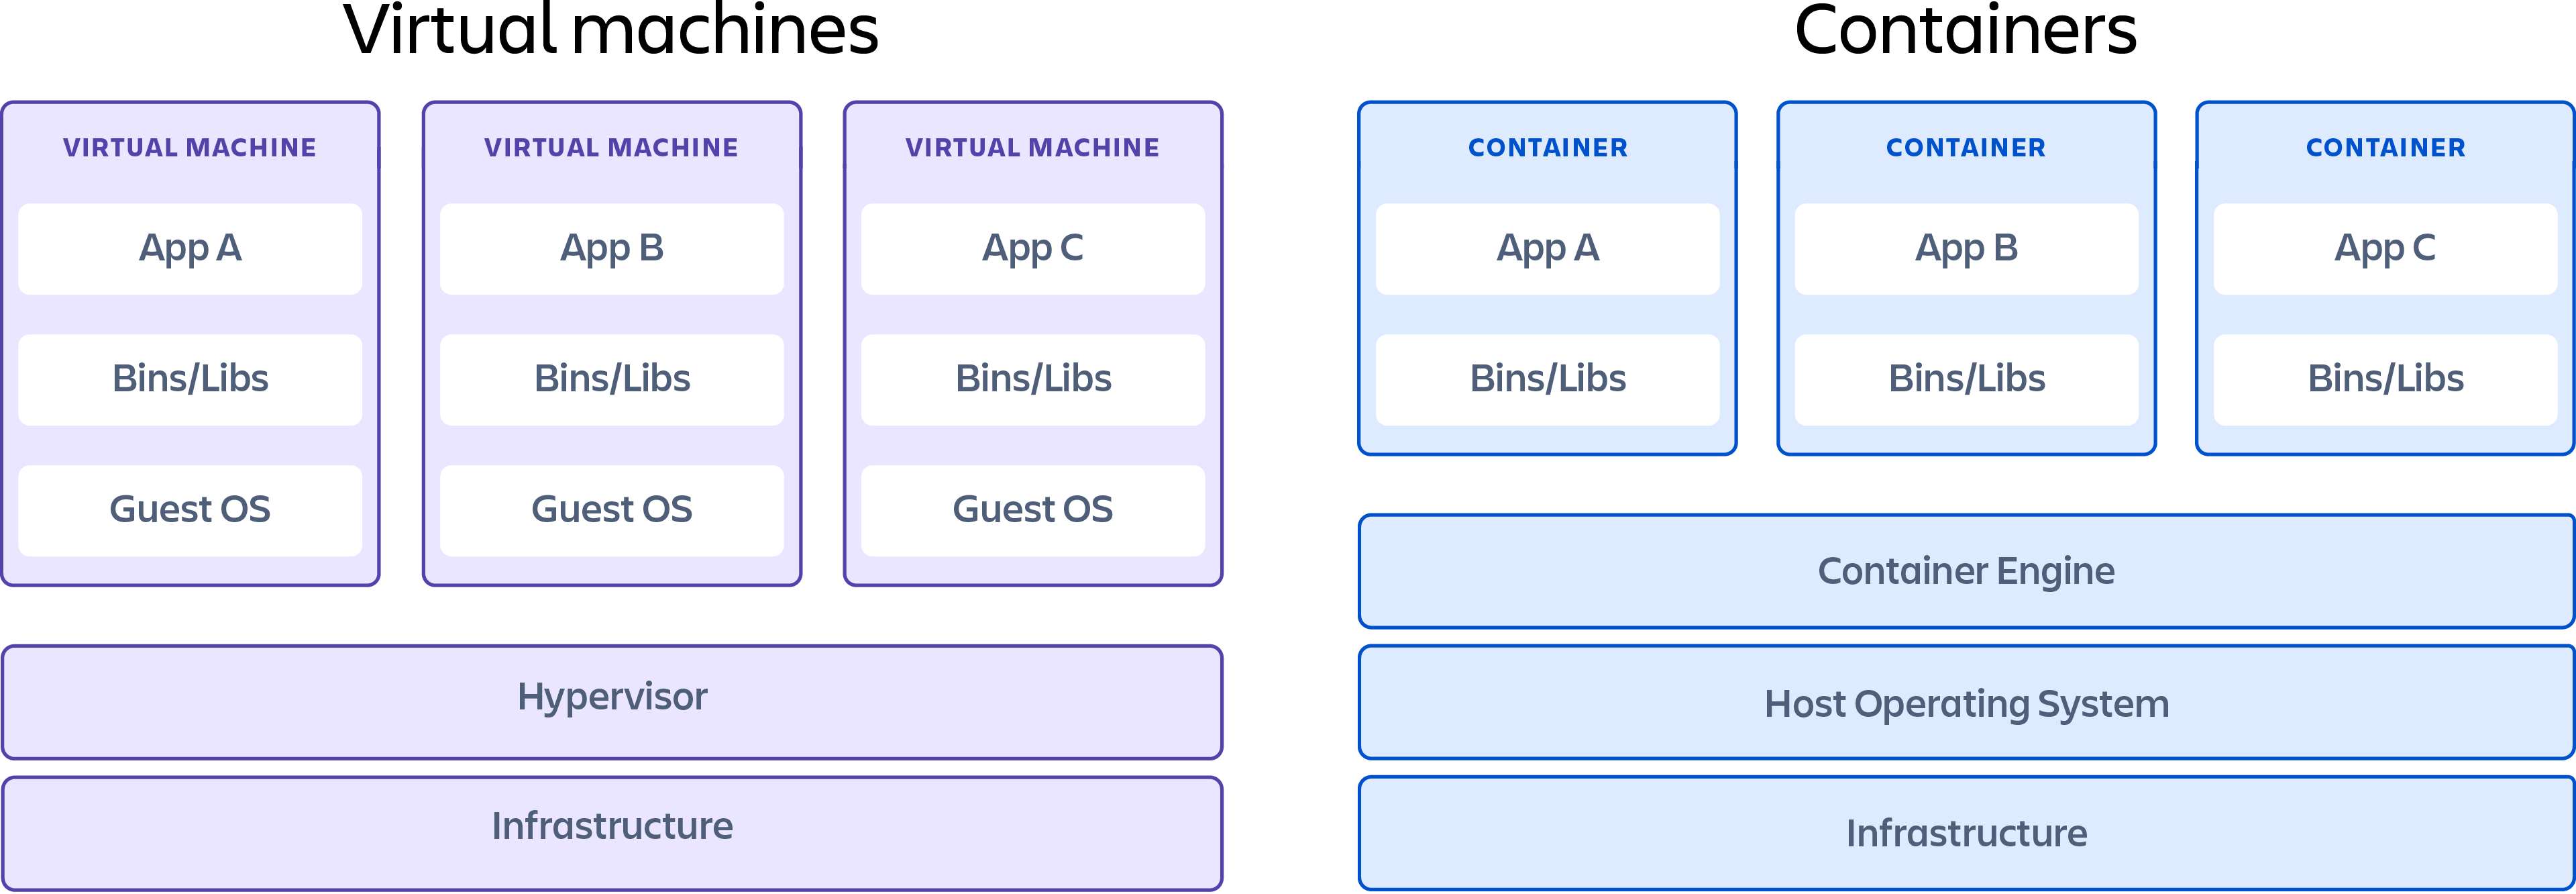
\includegraphics[width=120mm, keepaspectratio]{figures/virtudocker.png}
	\caption{Virtuális gépek és konténerek architekturális összehasonlítása.}
	\label{fig:virtudocker}
\end{figure}

A Docker egy konténerizációs fejlesztői környezet, a mélyén a \emph{containerd} névre keresztelt motor fut konténerizációs futtatókörnyezetként. \cite{Docker} Lehetővé teszi a konténerek létrehozását, indítását, kezelését és átvitelét. Virtuális tárhelyet és hálózatot biztosít a konténerek számára, és lehetővé teszi a konténerek közötti biztonságos kommunikációt. A Docker egy nyílt forráskódú projekt, amelyet a fejlesztők széles körben használnak a konténerizált alkalmazások fejlesztésére és futtatására.

\subsection{GitHub}

Szoftverrendszerek, alkalmazások fejlesztése során szinte elengedhetetlen a verziókezelés, amelynek segítségével a fejlesztők nyomonkövethetik a kódbázis változásait, visszaállíthatják az előző verziókat, és könnyen együtt tudnak dolgozni a kódon. Erre a munkafolyamatra az egyik legelterjedtebb Source Code Management (SCM) eszköz a Git verziókezelő. A Git egy elosztott verziókezelő rendszer. Minden fejlesztő saját gépén tárolja a teljes kódbázisát, majd a módosításokat a felhőben lévő tárolóval szinkronizálhatja.

A Git szoftver köré széleskörben találhatunk felhőtárhely-szolgáltatókat, ezek közül a legnépszerűbb a GitHub\footnote{\url{https://github.com/about}}. A GitHub a tárhelyen kívül sok más funkcionalitást is szolgáltat a hatékony együttműködés és kódgondozás kivitelezésére, egy ilyen szolgáltatása a GitHub Actions, amely CI/CD-folyamatok kezelésére egy eszköz, olyan folyamatokra hasznosítható, mint a statikus ellenőrzés, a build folyamatok automatizálása, és például a kód AWS-re való kiélesítése is.

\subsection{Terraform}

A Terraform\footnote{\url{https://www.terraform.io/}} egy elterjedt Infrastructure as Code (IaC) eszköz, amely lehetővé teszi a felhasználók számára, hogy infrastruktúrát definiáljanak kódban, és ezt az infrastruktúrát automatizáltan hozzák létre, módosítsák és töröljék. A Terraform a felhőszolgáltatók API-jait, illetve Cloud Development Kitjét (CDK) használja az változtatások érvényre juttatására. Go nyelven íródott a motorja, a Terraform IaC-ra pedig a saját HashiCorp Configuration Language (HCL) nyelvét ajánlja, amely egy deklaratív nyelv.
